\documentclass{article}
\usepackage[letterpaper,margin=1in]{geometry}
\usepackage{amsmath,booktabs,graphicx,float,longtable}
\usepackage[colorlinks=true,allcolors=blue]{hyperref}
\graphicspath{{../_output/}}
% Every number quoted in the text is a macro written by src/report_latex_tables.py.
\newcommand{\ScoreScored}{59}
\newcommand{\ScorePassed}{49}
\newcommand{\ScoreBand}{3}
\newcommand{\TrainRows}{65,752}
\newcommand{\ModelAUC}{0.635}
\newcommand{\PaperAUC}{0.708}
\newcommand{\AgreePearson}{0.55}
\newcommand{\AgreeRows}{125,982}
\newcommand{\AgreeStocks}{1,180}
\newcommand{\TenCoef}{0.0048}
\newcommand{\TenT}{2.88}
\newcommand{\ElevenAlpha}{0.17}
\newcommand{\ElevenAlphaT}{2.1}
\newcommand{\ImpAlpha}{0.20}
\newcommand{\FourDayZero}{0.122}
\newcommand{\FourDayZeroPaper}{0.095}
\newcommand{\IAFiveDayOne}{0.448}
\newcommand{\IAFiveEvents}{2,857}
\newcommand{\FigOneIti}{0.070}
\newcommand{\FigOneCtrl}{0.035}
\newcommand{\FigOnePaperIti}{0.146}
\newcommand{\ItradeOurs}{0.363}
\newcommand{\ItradePaper}{0.360}
\newcommand{\VolRatioMin}{0.834}
\newcommand{\MinCoverage}{0.64}
\newcommand{\MinCoverageYear}{2009}
\newcommand{\MinPearson}{0.52}


\title{Informed Trading Intensity: Replication and Extension}
\author{Jacob Lerner \and Andrew Arbitman \and Andrew McLaughlin \and Nate Lee}
\date{}

\begin{document}
\maketitle

\section{Project Overview}
\cite{bogousslavsky2024informed} train a gradient-boosted tree classifier to
recognize days on which Schedule 13D activists trade, using 41 same-day
liquidity, return, volatility and volume features. Applied to every stock-day,
the classifier's probability is the Informed Trading Intensity (ITI). The paper
shows that ITI detects informed trades better than standard liquidity
measures, rises around earnings and M\&A announcements, predicts weaker return
reversal, and predicts higher next-month returns.

We rebuilt the pipeline end to end on a shorter sample (2005--2019 instead of
1993--2019): we extracted 13D transaction labels from the original filing text,
constructed all 41 features from CRSP, WRDS Intraday Indicators and supplemental
TAQ aggregates, trained our own ITI(13D) with nested calendar-fold
cross-validation, and replicated the downstream exhibits. Because our sample is
shorter and our labels are reconstructed, we do not target exact equality. We
fixed one acceptance rule before comparing: an estimate matches if it has the
paper's sign and lies within a factor of \ScoreBand{} of the published value
(looser when the paper's own estimate is insignificant). By that rule,
\ScorePassed{} of \ScoreScored{} scored comparisons replicate
(Table~\ref{tab:scorecard}).

\paragraph{Where it worked.} The event-study exhibits (earnings, news, M\&A),
the return-reversal regression, ITI(impatient) return predictability, and the
stability of ITI's advantage over liquidity controls in Figure~1 replicate in
sign and magnitude. ITI(13D) return predictability replicates in sign, with
smaller magnitude for the long-short alpha (Table~11, 0.33 of the paper's).

\paragraph{Where it was hard.} (i) Raw 13D data: filers' transaction tables are
free text, so we wrote and hand-audited an extractor. (ii) TAQ: several of the
41 features are not in WRDS Intraday Indicators and required bounded server-side
TAQ aggregation. (iii) Our trained ITI(13D) reaches an out-of-sample ROC AUC of
\ModelAUC{} against the paper's \PaperAUC{}, and its yearly explanatory power is
about half the paper's. (iv) ITI(insider) and ITI(patient) lose most of their
return predictability in our 2005--2019 window.

\paragraph{Data sources.} CRSP daily stock, names, delisting and index files;
WRDS Intraday Indicators and TAQ; WRDS SEC filing text (Schedule 13D);
Compustat quarterly earnings dates; SDC M\&A; Thomson Reuters insider filings;
Markit securities lending; the authors' posted ITI series; the
Boudoukh--Feldman--Kogan--Richardson news classifications; and Kenneth French's
factors.

\section{Data and Validation}
Table~\ref{tab:validation} checks our data against benchmarks that do not depend
on our code. Panel A compares the rebuilt 13D labels with statistics published
in the paper: the share of window days with a 13D trade is \ItradeOurs{}
(paper: \ItradePaper{}), and filers trade more often in the last 20 days than
in the first 40, as the 10-day filing deadline implies. Panel B reconciles our
TAQ bucket-sum volume with WRDS Intraday Indicators (IID) market-hours volume
(lowest ratio \VolRatioMin{}).
Panel C and Figure~\ref{fig:validation} track coverage over time. Every
training year keeps at least \MinCoverage{} of label rows after the feature
screens (lowest in \MinCoverageYear{}), and our yearly ITI(13D) correlation with
the authors' posted series never falls below \MinPearson{}. These checks run
as tests in the pipeline (\texttt{tests/test\_data\_validation.py}).

\begin{table}[H]
\centering\small
\caption{Data validation. Rebuilt labels match the paper's trade frequency
closely, but filers' share of daily volume is about half the published figure.
Our extractor keeps small trades that the authors may have aggregated, so
our labels carry the right timing with a weaker per-day signal. Our TAQ volume
matches WRDS IID volume exactly in 2004 and is \VolRatioMin{} or more of it in 2019. Both
aggregate the same TAQ trades, so this checks our aggregation rather than the
trade data itself; the 2019 shortfall is volume printed under sale conditions
our regular/odd-lot screen excludes. Coverage and agreement with the
authors' series clear every tolerance, so differences in the downstream exhibits
do not come from a broken universe or a missing year.}
\label{tab:validation}
\resizebox{\textwidth}{!}{\begin{tabular}{lrrl}
\toprule
Check & Ours & Benchmark & Benchmark source \\
\midrule
\multicolumn{4}{l}{\textit{A. Rebuilt Schedule 13D labels (2005--2018) vs published statistics}} \\
Stock-days per filing & 40.993 & 36.533 & Table 1: 58,197 rows / 1,593 filings \\
Share of days with 13D trade & 0.363 & 0.360 & Table 1 \\
  ... first 40 days (patient) & 0.321 & 0.300 & Sec. 4.1: 30\% of days in first 40 \\
  ... last 20 days (impatient) & 0.440 & 0.490 & Sec. 4.1: 49\% of days in last 20 \\
Filer share of daily volume & 0.142 & 0.280 & Sec. 3.1: 28\% of daily volume when trading \\
  ... patient & 0.125 & 0.200 & Sec. 4.1 \\
  ... impatient & 0.167 & 0.370 & Sec. 4.1 \\
13D turnover, mean ($\times 100$) & 0.294 & 0.276 & Table IA.5, trade days \\
13D turnover, median ($\times 100$) & 0.078 & 0.105 & Table IA.5, trade days \\
Share of 13D trades that are sells & 0.120 & 0.060 & ITI\_main.py comment: $\sim$6\% of activist trades are sells \\
\midrule
\multicolumn{4}{l}{\textit{B. TAQ bucket sum vs WRDS IID volume (pilot days)}} \\
Volume ratio 2004 (3 stocks) & 1.000--1.000 & $\leq$ 1 & IID total\_vol\_m \\
Volume ratio 2019 (3 stocks) & 0.834--0.967 & $\leq$ 1 & IID total\_vol\_m \\
\midrule
\multicolumn{4}{l}{\textit{C. Coverage and agreement with the authors' posted ITI}} \\
Min.\ label rows with model inputs, 2005--2018 & 0.643 & $\geq$ 0.60 & tolerance \\
Min.\ scored days found in authors' file & 0.954 & $\geq$ 0.95 & tolerance \\
Min.\ yearly Pearson, ours vs authors' ITI(13D) & 0.519 & $\geq$ 0.40 & tolerance \\
Volume ratio band & 0.834--1.000 & 0.8--1.0 & tolerance \\
\bottomrule
\end{tabular}
}
\end{table}

\begin{figure}[H]
\centering
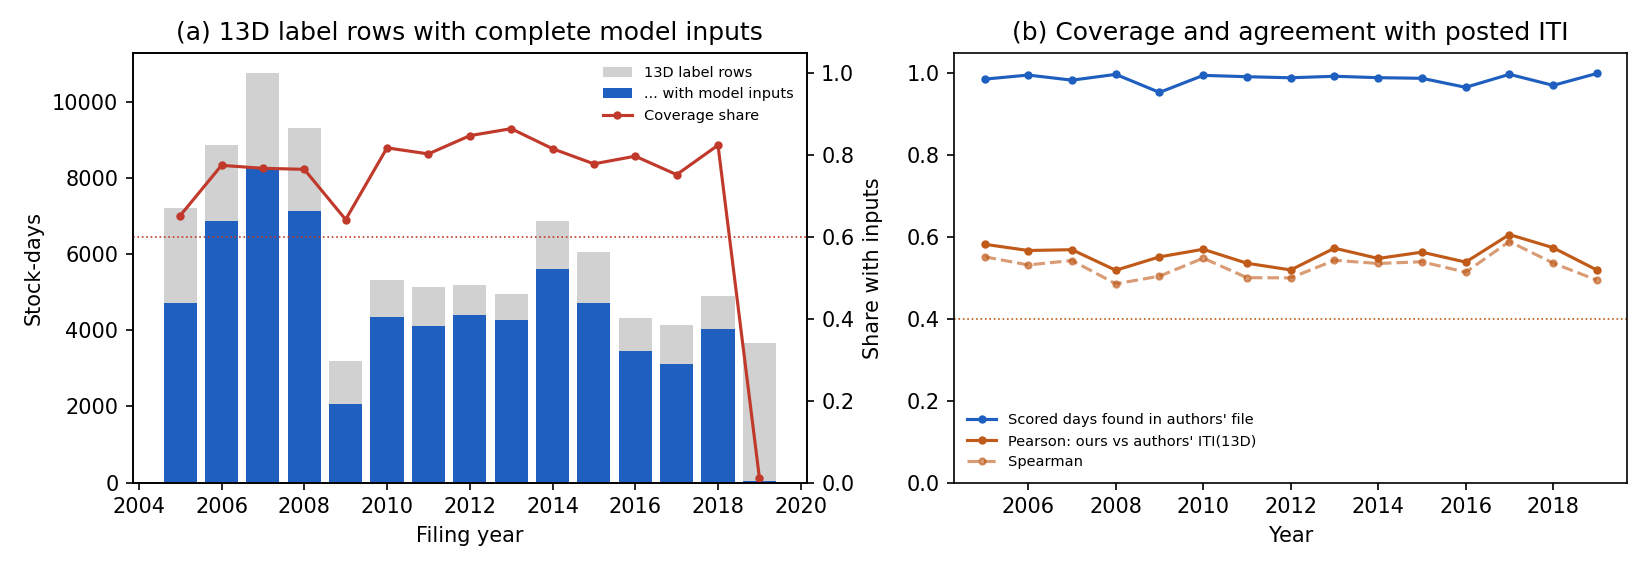
\includegraphics[width=\textwidth]{report/validation_coverage.png}
\caption{Coverage through time. (a) 13D label rows and those with all model
inputs; the dotted line is the 60\% tolerance. The 2019 drop is by design:
13D training ends in 2018, so we did not collect 2019 training inputs.
(b) Share of our scored stock-days present in the authors' posted file, and the
correlation between our ITI(13D) and theirs. There are no unexplained breaks,
and agreement is stable across market regimes.}
\label{fig:validation}
\end{figure}

\begin{figure}[H]
\centering
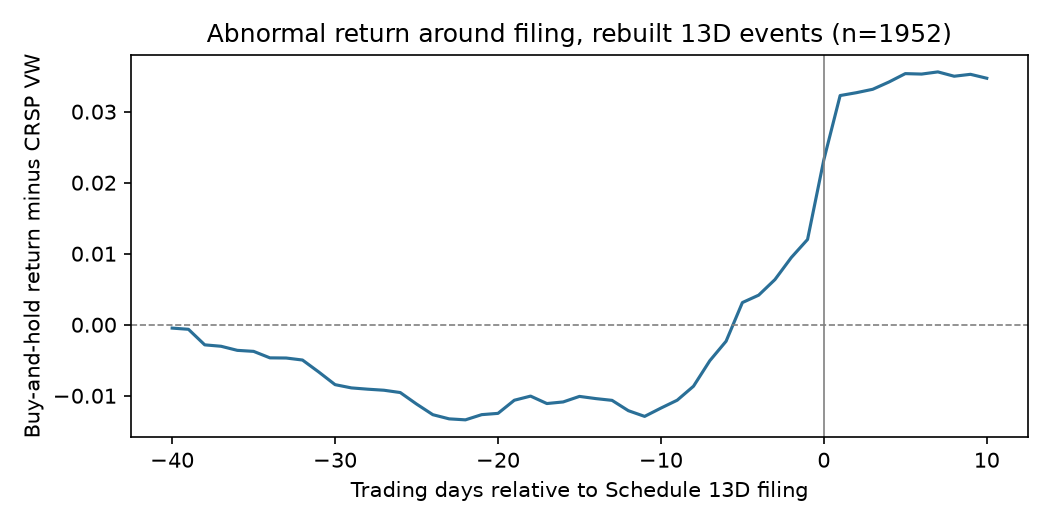
\includegraphics[width=0.7\textwidth]{13d_filing_car.png}
\caption{Cumulative abnormal return around our rebuilt 13D filings. The
two-day filing jump matches the paper's Figure IA.1 (about 2\%), confirming that
our filing dates and stock links are correct. The pre-filing run-up is smaller
than the paper's, consistent with our weaker per-day trade signal.}
\end{figure}

\section{Replication Results}

{\scriptsize
\setlength{\LTcapwidth}{\textwidth}
\def\ScorecardCaption{\caption{Replication scorecard. Each row compares one of our estimates with the
published value. ``Pass'' means the same sign and a ratio within
$[1/\ScoreBand, \ScoreBand]$ (or, when the paper's estimate is insignificant,
the same sign or also insignificant). \ScorePassed{} of \ScoreScored{}
comparisons pass. The failures concentrate in ITI(insider) and ITI(patient)
return predictability and in the volatility partial dependence of Figure~2.}\label{tab:scorecard}}
\begin{longtable}{llrrrl}
\ScorecardCaption \\
\toprule
Exhibit & Item & Ours & Paper & Ours/Paper & Status \\
\midrule
\endfirsthead
\toprule
Exhibit & Item & Ours & Paper & Ours/Paper & Status \\
\midrule
\endhead
Table 5 & col 1: ret & -0.0124 & -0.0040 & 3.10 & pass \\
 & col 2: ret & -0.0305 & -0.0140 & 2.18 & pass \\
 & col 2: ITI(13D) & 0.0013 & 0.0020 & 0.66 & pass \\
 & col 2: ret$\times$ITI(13D) & 0.0463 & 0.0310 & 1.49 & pass \\
 & col 3: ret & -0.0131 & -0.0060 & 2.19 & pass \\
 & col 3: ITI(13D) & 0.0013 & 0.0020 & 0.65 & pass \\
 & col 3: ret$\times$ITI(13D) & 0.0273 & 0.0340 & 0.80 & pass \\
 & col 3: ret$\times$turn & 0.0546 & 0.0080 & 6.83 & pass \\
 & col 3: ret$\times$rvol & -79.43 & -0.0290 & 2739.13 & not comparable \\
 & col 3: ret$\times$ES\% & -2.5363 & -0.7560 & 3.35 & fail \\
\midrule
Table 10 & col 1: ITI(13D) & 0.0048 & 0.0126 & 0.38 & pass \\
 & col 2: ITI(13D) & 0.0050 & 0.0117 & 0.42 & pass \\
 & col 2: ITI(insider) & 0.0011 & 0.0119 & 0.09 & fail \\
 & col 2: ITI(short) & -0.0018 & -0.0084 & 0.21 & pass \\
 & col 3: ITI(patient) & -0.0014 & 0.0006 & -2.29 & pass \\
 & col 3: ITI(impatient) & 0.0078 & 0.0158 & 0.50 & pass \\
 & col 4: ITI(13D) & 0.0025 & 0.0053 & 0.48 & pass \\
 & col 4: ITI(insider) & 0.0006 & 0.0107 & 0.05 & fail \\
 & col 4: ITI(short) & -0.0087 & -0.0201 & 0.44 & pass \\
 & col 4: ITI(patient) & -0.0027 & -0.0030 & 0.90 & pass \\
 & col 4: ITI(impatient) & 0.0090 & 0.0163 & 0.55 & pass \\
 & col 5: ITI(13D) & 0.0038 & 0.0061 & 0.62 & pass \\
 & col 5: ITI(insider) & 0.0034 & 0.0094 & 0.36 & pass \\
 & col 5: ITI(short) & -0.0153 & -0.0065 & 2.36 & pass \\
 & col 5: ITI(patient) & -0.0002 & -0.0038 & 0.06 & pass \\
 & col 5: ITI(impatient) & 0.0063 & 0.0164 & 0.39 & pass \\
\midrule
Table 11 & ITI(13D) H-L raw & 0.0015 & 0.0044 & 0.34 & pass \\
 & ITI(13D) H-L FF4 alpha & 0.0017 & 0.0052 & 0.33 & fail \\
 & ITI(insider) H-L raw & 0.0003 & 0.0037 & 0.09 & fail \\
 & ITI(insider) H-L FF4 alpha & -0.0001 & 0.0022 & -0.04 & fail \\
 & ITI(short) H-L raw & 0.0012 & 0.0014 & 0.88 & pass \\
 & ITI(short) H-L FF4 alpha & -0.0002 & 0.0005 & -0.32 & pass \\
 & ITI(patient) H-L raw & 0.0009 & 0.0030 & 0.29 & fail \\
 & ITI(patient) H-L FF4 alpha & 0.0010 & 0.0034 & 0.29 & fail \\
 & ITI(impatient) H-L raw & 0.0024 & 0.0051 & 0.47 & pass \\
 & ITI(impatient) H-L FF4 alpha & 0.0020 & 0.0054 & 0.38 & pass \\
\midrule
Figure 1 & mean annual adj. R2, ITI & 0.0700 & 0.1464 & 0.48 & pass \\
 & mean annual adj. R2, controls & 0.0353 & 0.0421 & 0.84 & pass \\
 & share of years ITI beats controls & 1.0000 & 1.0000 & 1.00 & pass \\
\midrule
Figure 2 & ITI change across volume range & 0.0764 & 0.1588 & 0.48 & pass \\
 & ITI change across volatility range & 0.0000 & -0.0683 & -0.00 & fail \\
\midrule
Table IA.6 & ROC AUC minus 0.5 & 0.1350 & 0.2084 & 0.65 & pass \\
\midrule
Figure 4(a) & day -2 & 0.0101 & 0.0050 & 2.02 & pass \\
 & day -1 & 0.0291 & 0.0180 & 1.62 & pass \\
 & day +0 & 0.1225 & 0.0950 & 1.29 & pass \\
 & day +1 & 0.0606 & 0.0440 & 1.38 & pass \\
 & day +2 & 0.0445 & 0.0340 & 1.31 & pass \\
\midrule
Figure 4(b) & large day -1 & 0.0372 & 0.0300 & 1.24 & pass \\
 & large day +0 & 0.1850 & 0.1550 & 1.19 & pass \\
 & large day +1 & 0.1105 & 0.0900 & 1.23 & pass \\
 & small day -1 & 0.0217 & 0.0060 & 3.61 & fail \\
 & small day +0 & 0.0861 & 0.0580 & 1.48 & pass \\
 & small day +1 & 0.0295 & 0.0140 & 2.11 & pass \\
\midrule
Figure 4(c) & day -1 & 0.0071 & 0.0063 & 1.13 & pass \\
 & day +0 & 0.0115 & 0.0120 & 0.96 & pass \\
 & day +1 & 0.0081 & 0.0065 & 1.25 & pass \\
\midrule
Figure IA.5 & day -1 & 0.0090 & 0.0235 & 0.38 & pass \\
 & day +0 & 0.3920 & 0.2700 & 1.45 & pass \\
 & day +1 & 0.4479 & 0.3070 & 1.46 & pass \\
 & day +5 & 0.2946 & 0.1790 & 1.65 & pass \\
\bottomrule
\end{longtable}

}

\begin{figure}[H]
\centering
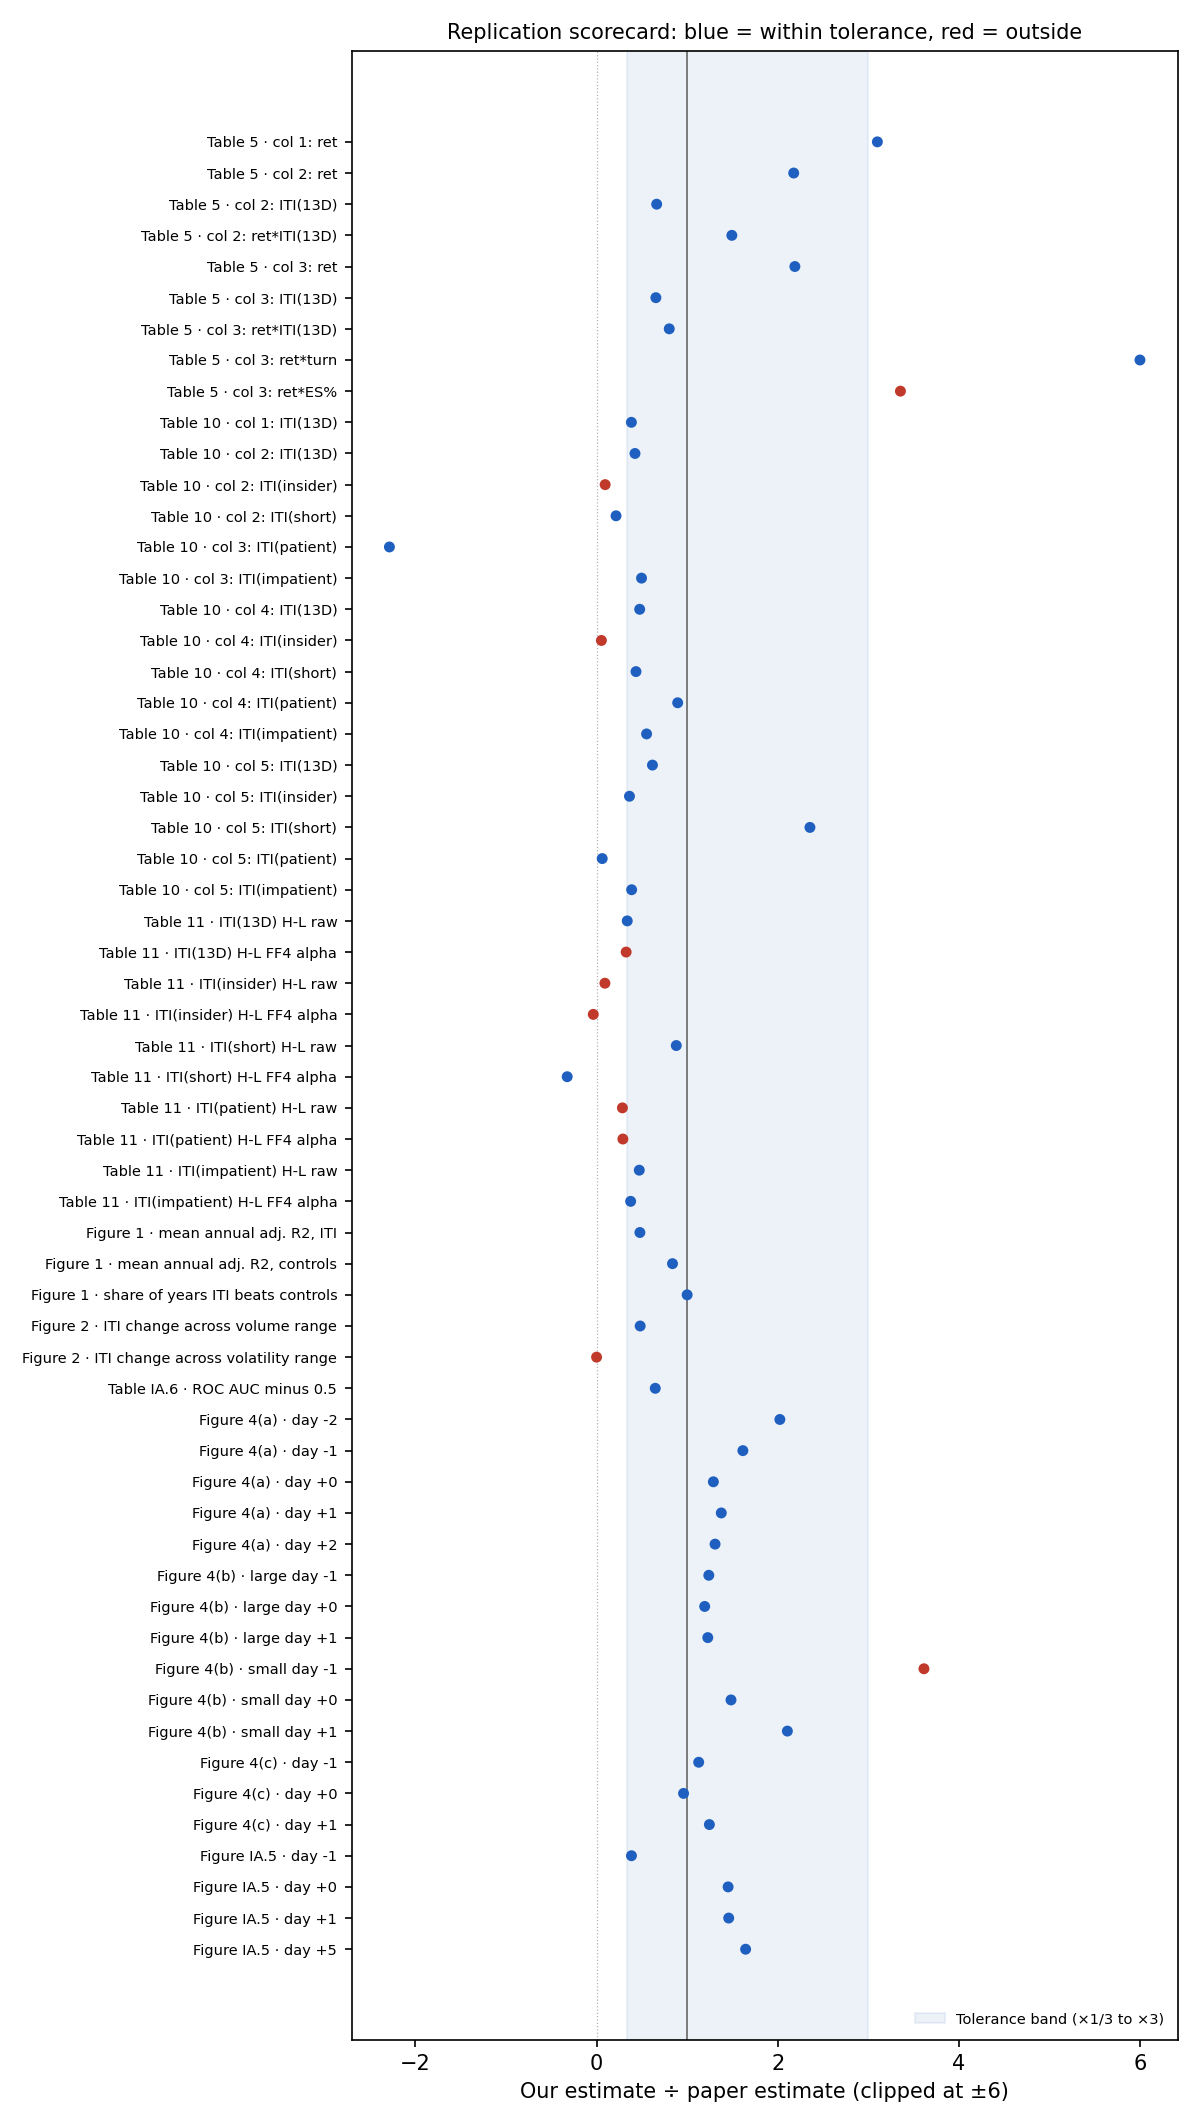
\includegraphics[width=0.85\textwidth,height=0.8\textheight,keepaspectratio]{report/scorecard.png}
\caption{Scorecard as ratios of our estimate to the paper's. Most points sit
inside the shaded tolerance band. Return-predictability estimates (Tables 10--11)
sit left of 1: right sign, smaller size, as expected from a model trained on a
shorter, reconstructed label sample. Event-study peaks (Figure 4, IA.5) sit at
or slightly right of 1. Of the points beyond the band at large ratios,
two pass because the paper's own estimate is insignificant (Table~5 \texttt{ret}
and \texttt{ret*turn}); two are genuine misses: Figure~4(b) ``small day $-1$''
(3.61, no published $t$-statistic) and Table~5 \texttt{ret*ES\%} (3.35, paper
$t=-4.94$).}
\end{figure}

\subsection{Detecting informed trading (Figures 1--3)}
\begin{figure}[H]
\centering
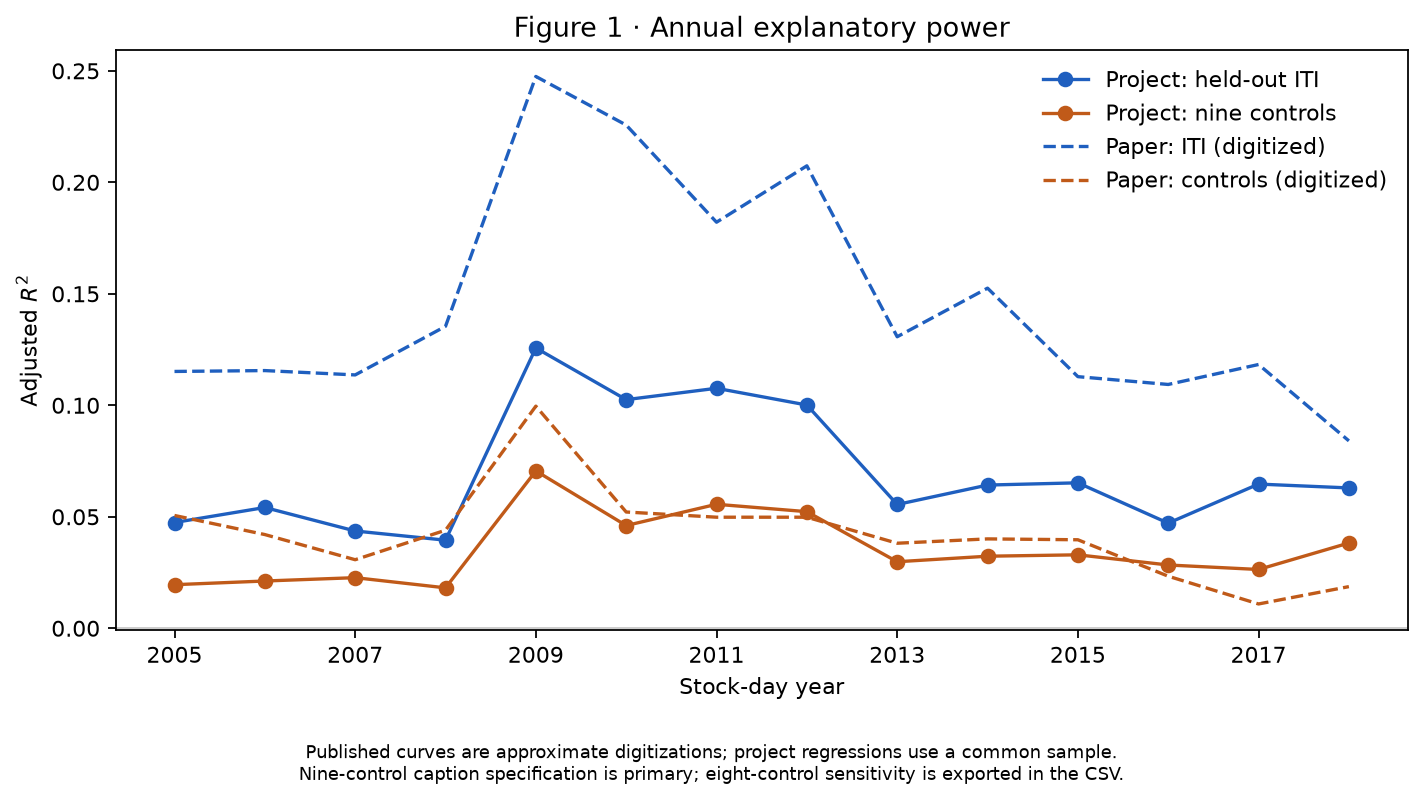
\includegraphics[width=0.8\textwidth]{replication/figure1.png}
\caption{Figure 1: annual out-of-sample adjusted $R^2$ for the 13D trade
indicator. Our ITI explains on average \FigOneIti{} per year versus
\FigOneCtrl{} for the liquidity controls, so ITI beats the controls in every year,
as in the paper. The level is about half the paper's (\FigOnePaperIti{}),
mirroring our lower AUC (\ModelAUC{} vs \PaperAUC{}).}
\end{figure}

\begin{figure}[H]
\centering
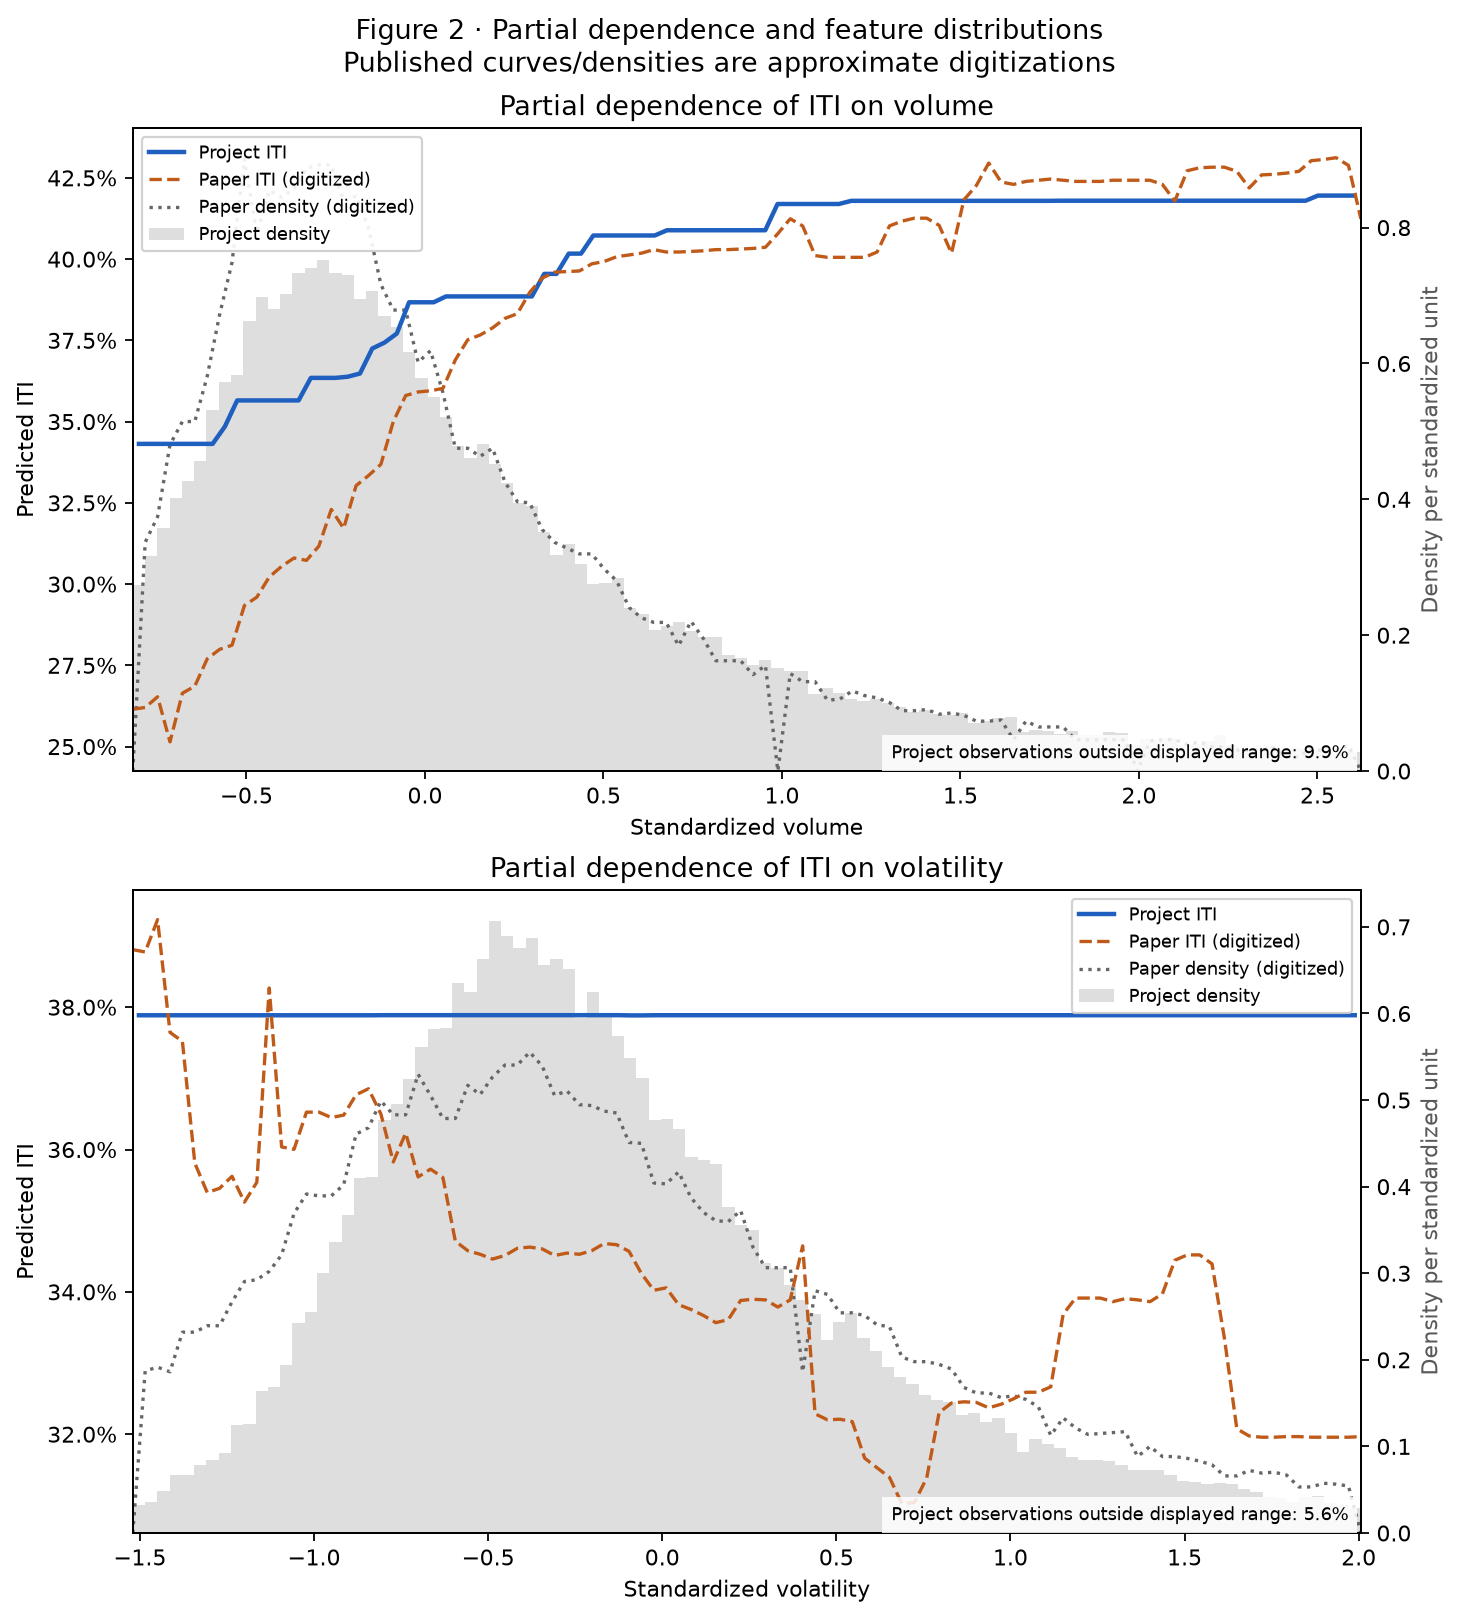
\includegraphics[width=0.6\textwidth]{replication/figure2.png}
\caption{Figure 2: partial dependence. ITI rises steeply and concavely in volume,
as in the paper. Our model is almost flat in volatility, where the paper finds a
decreasing, convex relation. This is the clearest difference between our
estimated model and the authors' model.}
\end{figure}

\begin{figure}[H]
\centering
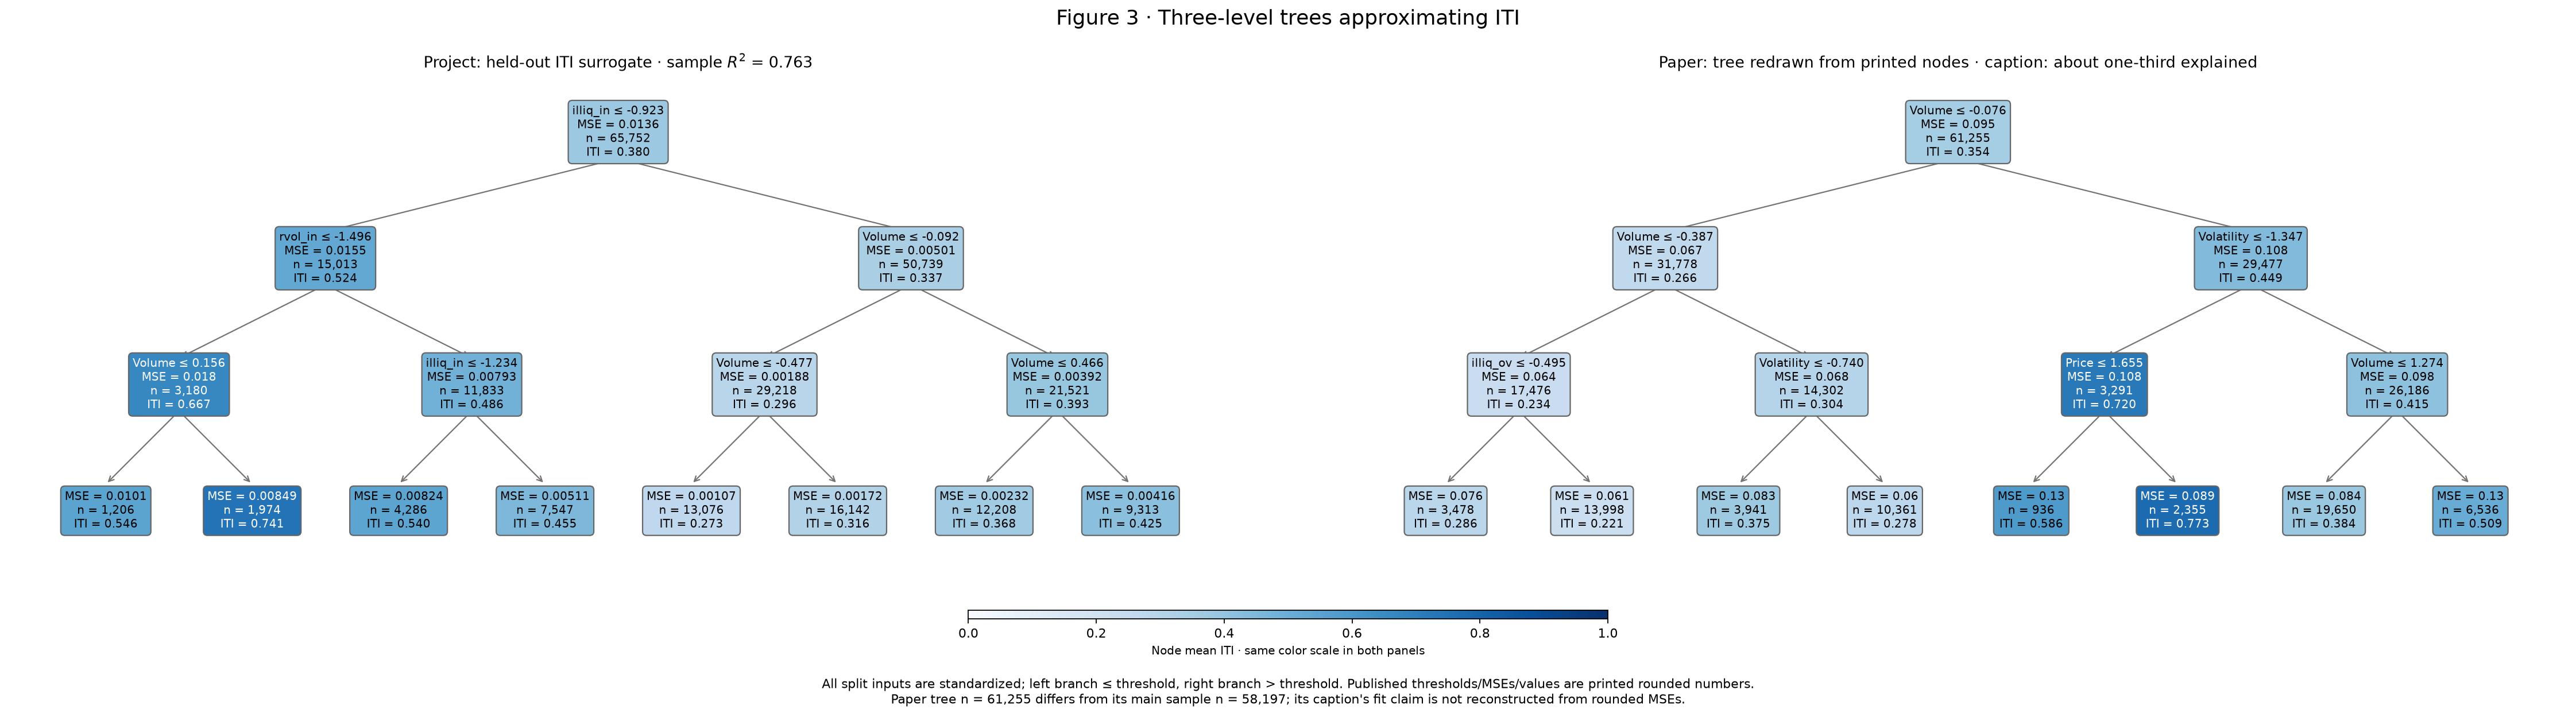
\includegraphics[width=\textwidth]{replication/figure3.png}
\caption{Figure 3: depth-3 surrogate tree approximating ITI. As in the paper,
volume appears repeatedly and high-volume/low-volatility days get the highest
ITI. Our tree splits first on intraday illiquidity rather than volume, a
reordering of the same ingredients.}
\end{figure}

\subsection{Return reversal (Table 5)}
\begin{table}[H]
\centering\scriptsize
\caption{Table 5: next-day return on today's return interacted with ITI(13D),
date fixed effects, stock/date clustered $t$-statistics. Returns on high-ITI days
reverse less ($\text{ret}\times\text{ITI}>0$), as the paper finds, and the
interaction survives the turnover, volatility and spread interactions. The
$\text{ret}\times\text{rvol}$ coefficient is not comparable because our
realized-volatility input has a different scale.}
\resizebox{\textwidth}{!}{\begin{tabular}{lrrrrrr}
\toprule
 & \multicolumn{2}{c}{(1)} & \multicolumn{2}{c}{(2)} & \multicolumn{2}{c}{(3)} \\
 & Ours & Paper & Ours & Paper & Ours & Paper \\
\midrule
ret & -0.012 & -0.004 & -0.030 & -0.014 & -0.013 & -0.006 \\
 & (-4.35) & (-1.77) & (-7.05) & (-4.48) & (-3.29) & (-1.98) \\
ITI(13D) &  &  & 0.001 & 0.002 & 0.001 & 0.002 \\
 &  &  & (13.33) & (23.55) & (12.58) & (20.00) \\
ret$\times$ITI(13D) &  &  & 0.046 & 0.031 & 0.027 & 0.034 \\
 &  &  & (7.36) & (6.45) & (4.50) & (5.83) \\
ret$\times$turn &  &  &  &  & 0.055 & 0.008 \\
 &  &  &  &  & (2.01) & (0.54) \\
ret$\times$rvol &  &  &  &  & -79.435 & -0.029 \\
 &  &  &  &  & (-2.04) & (-1.65) \\
ret$\times$ES\% &  &  &  &  & -2.536 & -0.756 \\
 &  &  &  &  & (-6.17) & (-4.94) \\
\midrule
Obs. & 9,567,779 &  & 9,567,779 &  & 9,318,834 &  \\
\bottomrule
\end{tabular}
}
\end{table}

\subsection{Informational events (Figure 4 and IA.5)}
\begin{figure}[H]
\centering
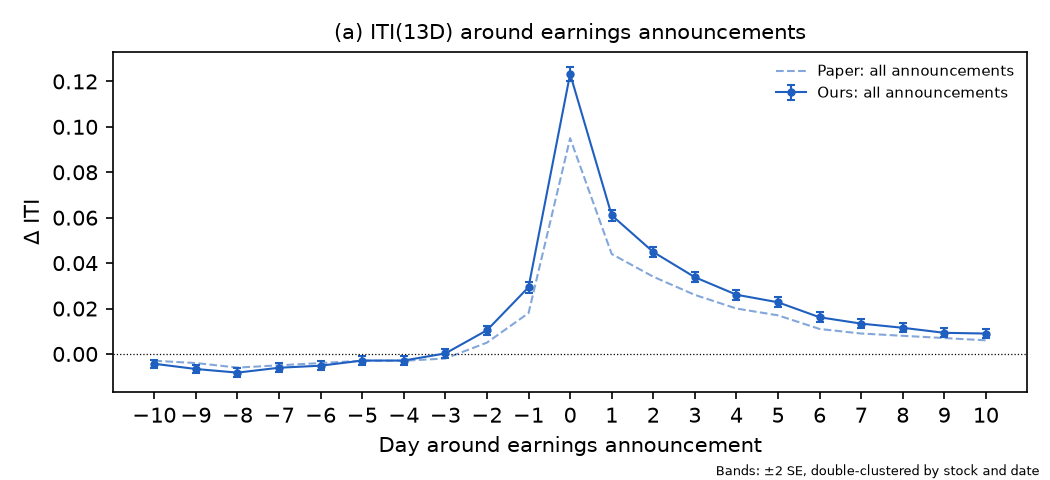
\includegraphics[width=0.85\textwidth]{replication/figure4a.png}
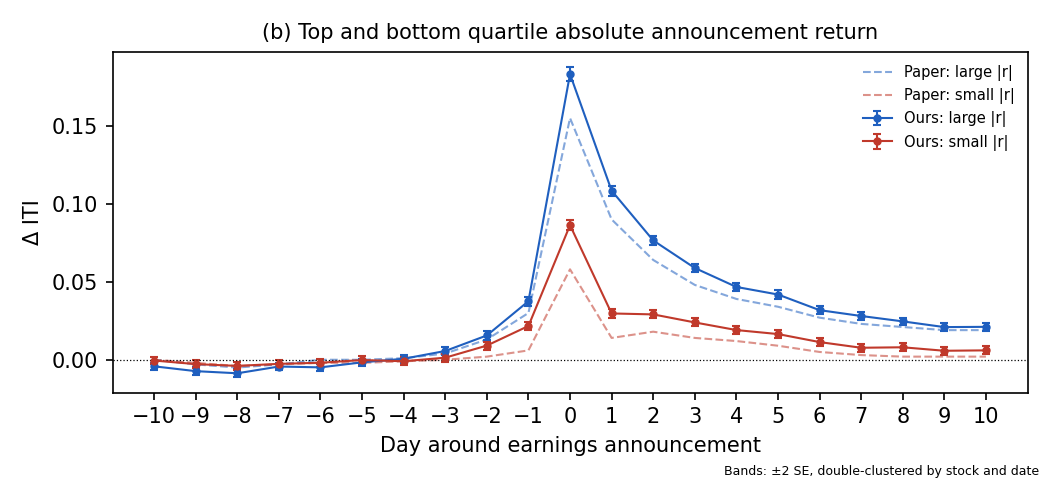
\includegraphics[width=0.85\textwidth]{replication/figure4b.png}
\caption{Figure 4(a)--(b): ITI(13D) around earnings announcements. ITI rises two
days before the announcement, peaks on day 0 (\FourDayZero{} vs the paper's
\FourDayZeroPaper{}), and stays elevated, most strongly for large-surprise
announcements. The pattern replicates closely.}
\end{figure}

\begin{figure}[H]
\centering
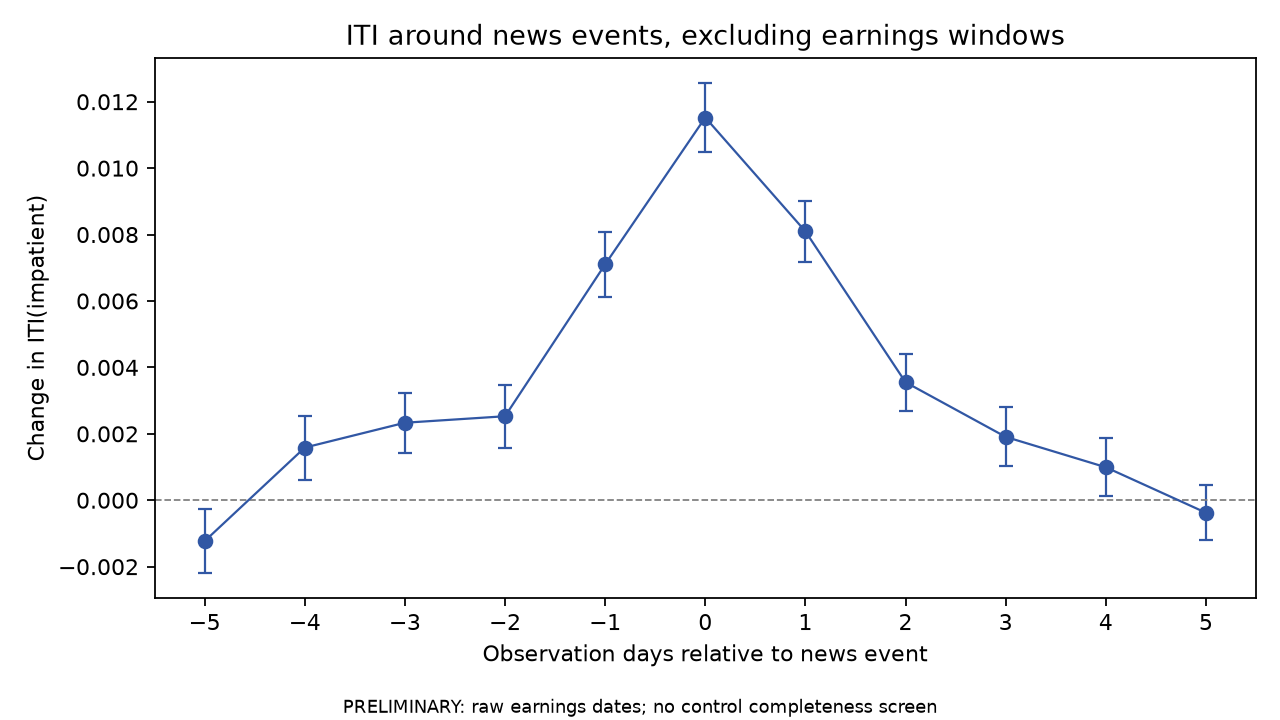
\includegraphics[width=0.75\textwidth]{figure_04c_preview.png}
\caption{Figure 4(c), preliminary: ITI around firm news days outside earnings
windows (BFKR news, 2005--2015). ITI rises the day before news and peaks on day
0, as in the paper. This version uses raw earnings dates for the exclusion
window and does not yet apply the full control screen.}
\end{figure}

\begin{figure}[H]
\centering
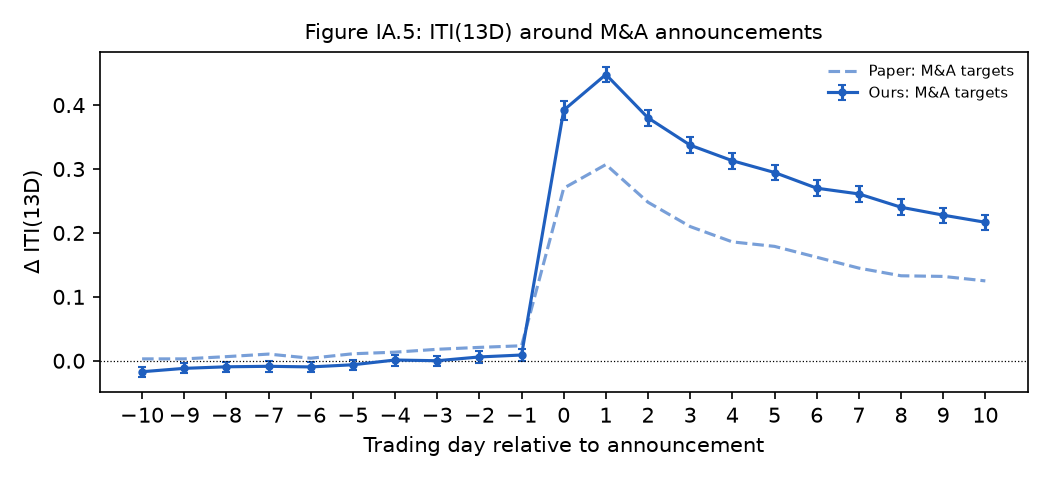
\includegraphics[width=0.85\textwidth]{replication/figureIA5.png}
\caption{Figure IA.5: ITI(13D) around M\&A announcements for public US targets
(\IAFiveEvents{} events). ITI jumps after the announcement (day +1:
\IAFiveDayOne{}) and decays, as in the paper. Our pre-announcement drift is weaker
and noisier.}
\end{figure}

\subsection{Asset pricing (Tables 10 and 11)}
\begin{table}[H]
\centering\scriptsize
\caption{Table 10: next-month return on prior-week ITI, week fixed effects,
stock/week clustered $t$-statistics. ITI(13D) predicts returns with a
coefficient of \TenCoef{} ($t=\TenT$), about 40\% of the paper's value, and
ITI(impatient) dominates ITI(patient), as in the paper. ITI(insider) does not
predict returns in our 2005--2019 window.}
\resizebox{\textwidth}{!}{\begin{tabular}{lrrrrrrrrrr}
\toprule
 & \multicolumn{2}{c}{(1)} & \multicolumn{2}{c}{(2)} & \multicolumn{2}{c}{(3)} & \multicolumn{2}{c}{(4)} & \multicolumn{2}{c}{(5)} \\
 & Ours & Paper & Ours & Paper & Ours & Paper & Ours & Paper & Ours & Paper \\
\midrule
ITI(13D) & 0.0048 & 0.0126 & 0.0050 & 0.0117 &  &  & 0.0025 & 0.0053 & 0.0038 & 0.0061 \\
 & (2.88) & (6.82) & (2.67) & (4.67) &  &  & (1.14) & (2.22) & (1.79) & (3.23) \\
ITI(insider) &  &  & 0.0011 & 0.0119 &  &  & 0.0006 & 0.0107 & 0.0034 & 0.0094 \\
 &  &  & (0.57) & (4.82) &  &  & (0.29) & (4.42) & (1.99) & (5.69) \\
ITI(short) &  &  & -0.0018 & -0.0084 &  &  & -0.0087 & -0.0201 & -0.0153 & -0.0065 \\
 &  &  & (-0.32) & (-1.29) &  &  & (-1.42) & (-2.79) & (-2.77) & (-1.26) \\
ITI(patient) &  &  &  &  & -0.0014 & 0.0006 & -0.0027 & -0.0030 & -0.0002 & -0.0038 \\
 &  &  &  &  & (-0.65) & (0.28) & (-1.26) & (-1.43) & (-0.11) & (-1.85) \\
ITI(impatient) &  &  &  &  & 0.0078 & 0.0158 & 0.0090 & 0.0163 & 0.0063 & 0.0164 \\
 &  &  &  &  & (3.20) & (6.51) & (2.99) & (5.83) & (2.22) & (5.25) \\
\midrule
Obs. & 1,913,001 &  & 1,913,001 &  & 1,913,001 &  & 1,913,001 &  & 1,913,001 &  \\
\bottomrule
\end{tabular}
}
\end{table}

\begin{table}[H]
\centering\scriptsize
\caption{Table 11: equal-weighted decile portfolios on prior-week ITI, monthly
percent returns, Newey--West $t$-statistics in parentheses. The ITI(13D)
high-minus-low FF4 alpha is \ElevenAlpha\% per month ($t=\ElevenAlphaT$) and
ITI(impatient)'s is \ImpAlpha\%. Both are positive and significant but about a third of
the paper's. ITI(short) is insignificant in both samples.}
\resizebox{\textwidth}{!}{\begin{tabular}{lrrrrrrrr}
\toprule
 & \multicolumn{4}{c}{Raw return} & \multicolumn{4}{c}{FF4 alpha} \\
\cmidrule(lr){2-5}\cmidrule(lr){6-9}
Sort variable & Low & High & H$-$L (ours) & H$-$L (paper) & Low & High & H$-$L (ours) & H$-$L (paper) \\
\midrule
ITI(13D) & 0.81 & 0.96 & 0.15 (1.8) & 0.44 (4.9) & -0.06 & 0.11 & 0.17 (2.1) & 0.52 (6.2) \\
ITI(insider) & 0.85 & 0.88 & 0.03 (0.4) & 0.37 (3.3) & -0.02 & -0.03 & -0.01 (-0.1) & 0.22 (2.9) \\
ITI(short) & 0.80 & 0.92 & 0.12 (1.0) & 0.14 (1.0) & 0.01 & -0.01 & -0.02 (-0.2) & 0.05 (0.5) \\
ITI(patient) & 0.87 & 0.96 & 0.09 (1.2) & 0.30 (3.9) & -0.00 & 0.10 & 0.10 (1.3) & 0.34 (4.2) \\
ITI(impatient) & 0.75 & 0.99 & 0.24 (2.6) & 0.51 (5.1) & -0.09 & 0.11 & 0.20 (2.2) & 0.54 (5.7) \\
\bottomrule
\end{tabular}
}
\end{table}

\section{Updated Results}
% TODO (update): rerun Tables 5, 10, 11 and Figure 4 through the latest data
% using the authors' extended ITI release (1993-2024) once CRSP 2020-2024 is
% collected. See TODO.md.
The update is in progress: the authors' refreshed ITI release runs through 2024,
and extending the panel requires CRSP and TAQ indicators for 2020--2024.

\section{Extension: a published ITI replication monitor}
Our extension is a ChartBook website, built by the pipeline and published on
GitHub Pages, that any researcher can use without WRDS access. It contains
(i) the replication scorecard, which recomputes automatically whenever an output
changes, (ii) a side-by-side comparison of our independently trained ITI(13D)
with the authors' posted series (overall correlation \AgreePearson{} on
\AgreeRows{} stock-days, \AgreeStocks{} stocks), with coverage diagnostics by
year, and (iii) the replicated exhibits with their data. Before using either
version of ITI, a researcher can see where the measure is robust (event
studies, reversal, ITI(13D) and ITI(impatient) pricing) and where it is fragile
(ITI(insider) pricing after 2005, volatility dependence).

\bibliographystyle{plain}
\bibliography{bibliography}
\end{document}
